%%%%%%%%%%%%%%%%%%%%%%%%%%%%%%%%%%%%%%%%%%%%%%%%%%%%%%%%%%%%%%%%%%%%%%%%%%%%%%%%
\documentclass[varwidth=true, border=70pt]{standalone}

\usepackage{tikz}
%\usepackage{standalone}

\usetikzlibrary{positioning,arrows,shapes,shadows}
\tikzstyle{format} = [draw, very thick, fill=blue!40]
\tikzstyle{medium} = [ellipse, draw=black, thick, fill=green!20, text=black]
\tikzstyle{qoi}=[rectangle, draw=black, rounded corners, fill=green, drop shadow]
\tikzstyle{cblue}=[circle, draw, thin,fill=blue!10, scale=0.8]
\tikzstyle{decision} = [diamond, draw, fill=blue!20, 
    text width=5.5em, text badly centered, minimum size=3.6cm, node distance=3cm, inner sep=0pt, draw=black, text=black]
    \tikzstyle{biggray}=[rectangle, draw=black, thin, fill=gray!20,
                                 anchor=south east, text width=10em,
                                 text height=5em, minimum width=10em,
                                 minimum height=5.5em, rounded
                                 corners=20pt]
\textwidth 16.0cm
\textheight 23.0cm
\topmargin -2cm
\headheight 0cm
\headsep 0cm
\topskip 0cm
\oddsidemargin 0.00cm
\evensidemargin 0.00cm
%\addtolength{\textheight}{1in}


%%%%%%%%%%%%%%%%%%%%%%%%%%%%%%%%%%%%%%%%%%%%%%%%%%%%%%%%%%%%%%%%%%%%%%%%%%%%%%%%

\begin{document}
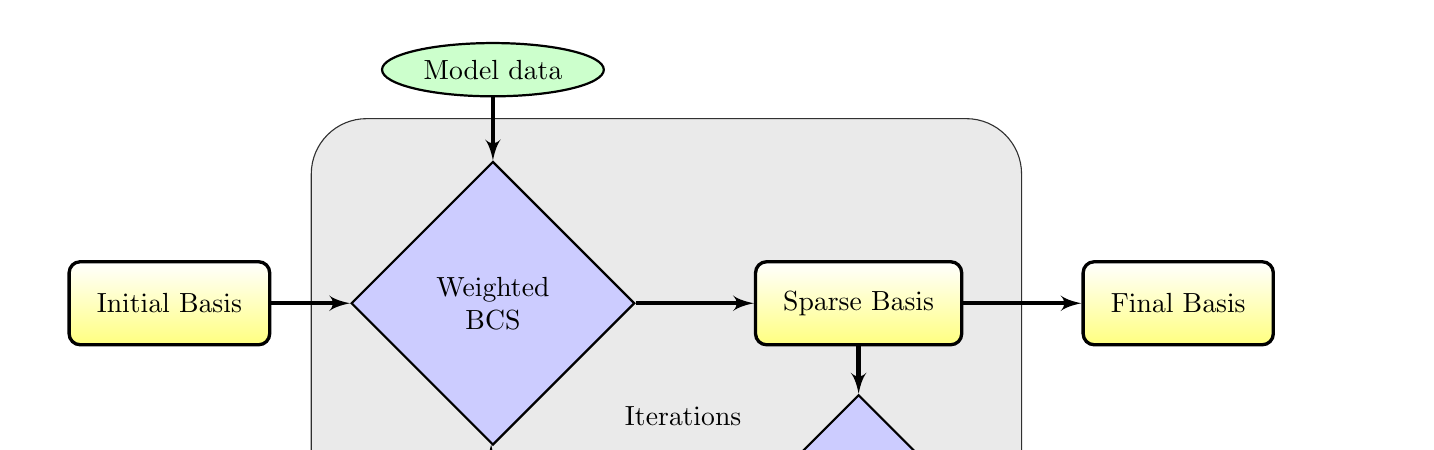
\begin{tikzpicture}[node distance=3cm, auto, thick]
\tikzset{
    mynode/.style={rectangle,rounded corners,draw=black, top color=white, bottom color=yellow!50,very thick, inner sep=1em, minimum size=3em, text centered, text=black},
    mynode2/.style={rectangle,rounded corners,draw=black, top color=white, bottom color=green!50,very thick, inner sep=1em, minimum size=3em, text centered, text=black},
    myarrow/.style={->, >=latex', shorten >=0pt, ultra thick,color=black},
    mylabel/.style={text width=7em, text centered, black} 
}  
    % We need to set at bounding box first. Otherwise the diagram
    % will change position for each frame.
    \path[use as bounding box] (-2.5,0) rectangle (15,5);
     \path[->] node[mynode] at (-0.7,1.5) (alpha){Initial Basis};
        \path[->] node[biggray, below right=-2.9 and 0.5 of alpha,opacity=0.8,text width=25em, text height=21em](cmod) {}
             node[mylabel, below left=-4.1 and -8.2 of cmod, text width=19em](pmod){Iterations};
     \path[->] node[decision, right=1.0 of alpha] (xds) {Weighted BCS }
                           (alpha) edge  [myarrow](xds);
    \path[->] node[medium, above=0.8 of xds] (prior) {Model data}
                      (prior) edge [myarrow] (xds);
    \path[->] node[mynode, right=1.5 of xds] (lam) {Sparse Basis}
                               (xds) edge [myarrow] (lam);
       \path[->] node[mynode, right=1.5 of lam] (fin) {Final Basis}
                               (lam) edge [myarrow] (fin);
\path[->] node[decision, below=0.6 of lam] (gr) {Basis Growth and Reweighting}
       (lam) edge  [myarrow](gr);
    \path[->] node[mynode, left=1.7 of gr] (fi) {New Basis}
                     (gr) edge [myarrow](fi)
               (fi) edge[myarrow]  (xds);
    \end{tikzpicture}
\end{document}

